\documentclass[letterpaper]{article}
    \usepackage{amsmath}
    \usepackage{tikz}
    \usepackage{epigraph}
    \usepackage{float}
    \usepackage{lipsum}
    \usepackage{glossaries}
    \usepackage{graphicx}
    \usepackage{imakeidx}
    \usepackage{hyperref}
    \usepackage{listings}
    \usepackage{color}
    \usepackage{csvsimple}
    \usepackage{lscape}

    \definecolor{codegreen}{rgb}{0,0.6,0}
    \definecolor{codegray}{rgb}{0.5,0.5,0.5}
    \definecolor{codepurple}{rgb}{0.58,0,0.82}
    \definecolor{backcolour}{rgb}{0.95,0.95,0.92}

    \lstdefinestyle{mystyle}{
        backgroundcolor=\color{backcolour},
        commentstyle=\color{codegreen},
        keywordstyle=\color{red},
        numberstyle=\tiny\color{codegray},
        stringstyle=\color{codepurple},
        basicstyle=\footnotesize,
        breakatwhitespace=false,
        breaklines=true,
        captionpos=b,
        keepspaces=true,
        numbers=left,
        numbersep=5pt,
        showspaces=false,
        showstringspaces=false,
        showtabs=false,
        tabsize=2
    }

    \lstset{style=mystyle}
    \graphicspath{{Images/}}
    \setcounter{tocdepth}{2}
    \makeglossaries
    \makeindex[columns=2, title=Alphabetical Index]
    \renewcommand\epigraphflush{flushright}
    \renewcommand\epigraphsize{\normalsize}
    \setlength\epigraphwidth{0.7\textwidth}

    \definecolor{titlepagecolor}{cmyk}{1,.60,0,.40}

    \DeclareFixedFont{\titlefont}{T1}{ppl}{b}{it}{0.5in}

    \makeatletter
    \def\printauthor{%
        {\large \@author}}
    \makeatother
    \author{
      Luke Duhe \\
      JJ Juarez \\
      Drake Lambert \\
      Kevin Phan \\
      Sam Miller \\
      Tristan Miller \\
      Timothy Ratliff \\
      Steven Vondenstein \\
      William Woodfin \\
       }

    % The following code is borrowed from:  https://tex.stackexchange.com/a/86310/10898

    \newcommand\titlepagedecoration{
    \begin{tikzpicture}[remember picture,overlay,shorten >= -10pt]

    \coordinate (aux1) at ([yshift=-15pt]current page.north east);
    \coordinate (aux2) at ([yshift=-410pt]current page.north east);
    \coordinate (aux3) at ([xshift=-4.5cm]current page.north east);
    \coordinate (aux4) at ([yshift=-150pt]current page.north east);

    \begin{scope}[titlepagecolor!40,line width=12pt,rounded corners=12pt]
    \draw
      (aux1) -- coordinate (a)
      ++(225:5) --
      ++(-45:5.1) coordinate (b);
    \draw[shorten <= -10pt]
      (aux3) --
      (a) --
      (aux1);
    \draw[opacity=0.6,titlepagecolor,shorten <= -10pt]
      (b) --
      ++(225:2.2) --
      ++(-45:2.2);
    \end{scope}
    \draw[titlepagecolor,line width=8pt,rounded corners=8pt,shorten <= -10pt]
      (aux4) --
      ++(225:0.8) --
      ++(-45:0.8);
    \begin{scope}[titlepagecolor!70,line width=6pt,rounded corners=8pt]
    \draw[shorten <= -10pt]
      (aux2) --
      ++(225:3) coordinate[pos=0.45] (c) --
      ++(-45:3.1);
    \draw
      (aux2) --
      (c) --
      ++(135:2.5) --
      ++(45:2.5) --
      ++(-45:2.5) coordinate[pos=0.3] (d);
    \draw
      (d) -- +(45:1);
    \end{scope}
    \end{tikzpicture}%
    }


% End borrowed code

\begin{document}
\begin{titlepage}

	\noindent
	\titlefont   "Ollert \par
	\epigraph{Project Report\\ November 30, 2018}%
	{\textit{}\\ \textsc{}}
	\null\vfill
	\vspace*{1cm}
	\noindent
	\hfill
	\begin{minipage}{0.35\linewidth}
		\begin{flushright}
			\printauthor
		\end{flushright}
	\end{minipage}
	%
	\begin{minipage}{0.02\linewidth}
		\rule{1pt}{125pt}
	\end{minipage}
	\titlepagedecoration
\end{titlepage}
\tableofcontents
\pagebreak
%Begin our document--------------------------------
\section{Database Design}
\subsection{Introduction}
Ollert is the backend database for a Kanban Board application (similar to https://Trello.com). It supports multiple users collaborating on one or many boards, through comments and task generation.

\pagebreak
\subsection{ER Diagram}
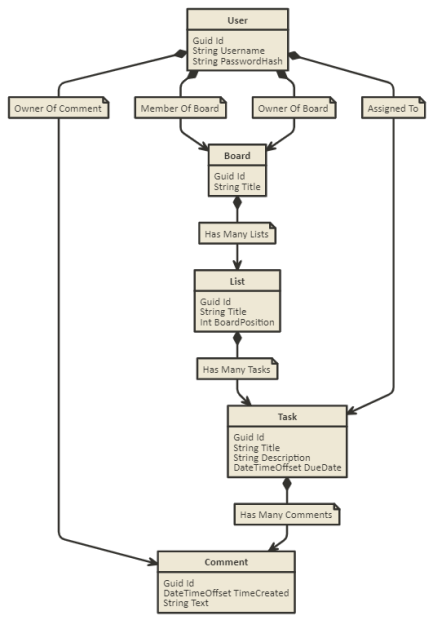
\includegraphics[scale=0.75]{Images/ER}
\pagebreak

\subsection{Identified Constraints}
\begin{itemize}
  \item{Every application user must have both a username and a password}
  \item{Usernames must be unique}
  \item{Every board must have a title and must be associated with an existing owner}
  \item{Every comment must have an owner}
  \item{Every comment must have a time and text}
  \item{Every comment must be associated with an existing task}
  \item{Every list must have a title and must be associated with an existing board}
  \item{Every task must be associated with an existing list}
  \item{Every entity in every table has a unique id}
\end{itemize}


\subsection{Assumptions About the Domain}
  \begin{itemize}
    \item Users should only have access to the boards they are members of
  \end{itemize}

\subsection{Database Design Process}

\subsection{Ollert's tables}
\subsubsection{Functional Dependencies}

\subsubsection{Primary Keys}
\begin{itemize}
  \item ApplicationUser
    \begin{itemize}
      \item ApplicationUser.Id
    \end{itemize}
  \item Board
    \begin{itemize}
      \item Board.Id
    \end{itemize}
  \item BoardMember
    \begin{itemize}
      \item none
    \end{itemize}
  \item List
    \begin{itemize}
      \item List.Id
    \end{itemize}
  \item Task
    \begin{itemize}
      \item Task.Id
    \end{itemize}
  \item TaskAssignee
    \begin{itemize}
      \item none
    \end{itemize}
  \item Comment
    \begin{itemize}
      \item Comment.Id
    \end{itemize}
\end{itemize}

\subsubsection{Foreign Keys}
\begin{itemize}
  \item Board
  \begin{itemize}
    \item ApplicationUser.Id
  \end{itemize}
  \item BoardMember
    \begin{itemize}
      \item Board.Id
      \item ApplicationUser.Id
    \end{itemize}
  \item List
    \begin{itemize}
      \item Board.Id
    \end{itemize}
  \item Task
    \begin{itemize}
      \item List.Id
    \end{itemize}
  \item TaskAssignee
    \begin{itemize}
      \item Task.Id
      \item ApplicationUser.Id
    \end{itemize}
  \item Comment
    \begin{itemize}
      \item Task.Id
      \item ApplicationUser.Id
    \end{itemize}
\end{itemize}
\pagebreak

%-----------------------Part 2 ----------------------------------------
\section{Database Implementation}

\subsection{Create Table Statements}
    \begin{lstlisting}[language=SQL, caption=ApplicationUser Table Creation Statement]
      create table ApplicationUser(
        Id char(32),
        Username varchar(100) not null,
        Passwordhash varchar(100) not null,
        primary key ( Id )
      );
    \end{lstlisting}

    \begin{lstlisting}[language=SQL, caption=Board Table Creation Statement]
      create table Board(
        Id char(32),
        Title varchar(100) not null,
        OwnerId char(32),
        primary key ( id ),
        foreign key ( OwnerId ) references ApplicationUser( Id )
      );
    \end{lstlisting}

    \begin{lstlisting}[language=SQL, caption=BoardMember Table Creation Statement]
      create table BoardMember(
        BoardId char(32),
        MemberId char(32),
        foreign key ( BoardId ) references Board( Id ),
        foreign key ( MemberId ) references ApplicationUser( Id )
      );
    \end{lstlisting}
    \begin{lstlisting}[language=SQL, caption=List Table Creation Statement]
      create table List(
        Id char(32),
        Title varchar(100) not null,
        BoardPosition int not null,
        BoardId char(32),
        primary key ( id ),
        foreign key ( BoardId ) references Board( Id )
      );
    \end{lstlisting}
    \begin{lstlisting}[language=SQL, caption=Task Table Creation Statement]
      create table Task(
        Id char(32),
        Title varchar(100) not null,
        Descriptor varchar(500) not null,
        DueDate datetimeoffset,
        ListId char(32),
        primary key ( id ),
        foreign key ( ListId ) references List( Id )
      )
    \end{lstlisting}
    \begin{lstlisting}[language=SQL, caption=TaskAssignee Table Creation Statement]
      create table TaskAssignee(
        TaskId char(32),
        AssigneeId char(32),
        foreign key ( TaskId ) references Task( Id ),
        foreign key ( AssigneeId ) references ApplicationUser( Id )
      )
    \end{lstlisting}
    \begin{lstlisting}[language=SQL, caption=Comment Table Creation Statement]
      create table Comment(
        Id char(32),
        TimeCreated datetimeoffset not null,
        MessageText varchar(100) not null,
        TaskId char(32),
        OwnerId char(32),
        primary key ( id ),
        foreign key ( TaskId ) references Task( Id ),
        foreign key ( OwnerId ) references ApplicationUser( Id )
      )
    \end{lstlisting}
%==============================================================================
\subsection{Insert Statements}
\begin{lstlisting}[language=SQL, caption=ApplicationUser Insert Statements]
  insert into ApplicationUser values ("19843875-6077-49", "Walter	Rogers",
   "168E5F6A717237FB2232A8AFE2DAAE3F8D582C5D4CC0EAA268F05F420F1EC421");

  insert into ApplicationUser values ("372a9ad5-4952-44", "Jean Bryant",
   "DAB12D7BB613EAC0304D9917738729FB37B60EBB1FB59FC9493ED64733CCE3BA");
\end{lstlisting}
\begin{lstlisting}[language=SQL, caption=Board Insert Statements]
  insert into Board values ("bbdd7100-cd10-41", "Sports Forum Mobile App", "19843875-6077-49");

  insert into Board values ("62376bd0-6ecc-4f", "Untitled Platformer Game", "372a9ad5-4952-44");
\end{lstlisting}
\begin{lstlisting}[language=SQL, caption=BoardMember Insert Statements]
  insert into BoardMember values ("fdd8f8a8-0d53-4f", "19843875-6077-49");

  insert into BoardMember values ("bbdd7100-cd10-41", "372a9ad5-4952-44");
\end{lstlisting}
\begin{lstlisting}[language=SQL, caption=List Insert Statements]
  insert into List values ("64251244-40f5-45","Admin Website", 2, "bbdd7100-cd10-41");

  insert into List values ("a583557a-3d83-4a","Art Design", 0, "62376bd0-6ecc-4f");
\end{lstlisting}
\begin{lstlisting}[language=SQL, caption=Task Insert Statements]
  insert into Task values ("e01479d6-6019-4a", "Database Design", "Design a robust database schema for storing all the data in our app.", "20180120 09:00:00 +10:00", "0e72d679-da23-41");

  insert into Task values ("d46993c0-ce64-46", "Story Design", "Write a fun story for the game.", "20180620 09:00:00 +10:00", "a583557a-3d83-4a");

\end{lstlisting}
\begin{lstlisting}[language=SQL, caption=TaskAssignee Insert Statements]
  insert into TaskAssignee values ("ac1a2b65-d1fc-47","88b03172-135a-4b");

  insert into TaskAssignee values ("a9f5ae59-6193-40","d263667b-ea46-4b");
\end{lstlisting}
\begin{lstlisting}[language=SQL, caption=Comment Insert Statements]
  insert into Comment values("c088cfa0-15e2-4f", "20180110 08:54:00 +10:00", "I'm probably going to need some help with this.", "e01479d6-6019-4a", "372a9ad5-4952-44");

  insert into Comment values("59646b1b-a084-49", "20180120 08:54:00 +10:00", "So I'm thinking our game has a mario-like character - but green.", "a9f5ae59-6193-40", "d263667b-ea46-4b");
\end{lstlisting}
\pagebreak

%==============================================================================

\subsection{Data Tables}
Due to the length of some of our fields the results may be split into multiple tables to fit on the page. Tables in the same horizontal rule pair are part of the same table.\\

\hrule
ApplicationUser Table
\csvautolongtable{application_user.csv}
\csvautolongtable{application_user1.csv}
\hrule
Board Table
\csvautolongtable{Board.csv}
\pagebreak
\hrule
Board Member Table
\csvautolongtable{board_member.csv}
\hrule
List Table
\csvautolongtable{list.csv}
\hrule
Task Table
\csvautolongtable{Task2.csv}
\csvautolongtable{Task.csv}
\csvautolongtable{Task1.csv}
\hrule
TaskAssignee Table
\csvautolongtable{task_assignee.csv}
\hrule
Comment Table
\csvautolongtable{comment1.csv}
\csvautolongtable{comment.csv}
\csvautolongtable{comment2.csv}
\hrule
\pagebreak
%=======================================================================
\subsection{Data manipulation statements}

\subsubsection{Select statements}

\begin{figure}[H]
\centering
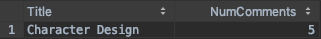
\includegraphics[scale=0.5]{Images/MostActiveTask-Comments}
\end{figure}
\begin{lstlisting}[language=SQL, caption=Select Most Active Task (Comments)]
SELECT TOP 1 Title, Count(*) as NumComments FROM Task, Comment WHERE Task.Id=Comment.TaskId GROUP BY Title ORDER BY NumComments DESC;
\end{lstlisting}
\hrule
\begin{figure}[H]
\centering
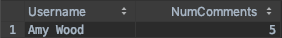
\includegraphics[scale=0.5]{Images/MostActiveUser-Comments}
\end{figure}
\begin{lstlisting}[language=SQL, caption=Select Most Active User (Comments)]
SELECT TOP 1 Username, Count(*) as NumComments FROM ApplicationUser, Comment WHERE ApplicationUser.Id=Comment.OwnerId GROUP BY Username ORDER BY NumComments desc;
\end{lstlisting}
\hrule
\begin{figure}[H]
\centering
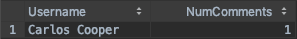
\includegraphics[scale=0.5]{Images/LeastActiveUser-Comments}
\end{figure}
\begin{lstlisting}[language=SQL, caption=Select Least Active User (Comments)]
SELECT TOP 1 Username, COUNT(*) as NumComments FROM Comment, ApplicationUser WHERE ApplicationUser.Id = Comment.OwnerId GROUP BY Username ORDER BY NumComments ASC;
\end{lstlisting}
\hrule
\begin{figure}[H]
\centering
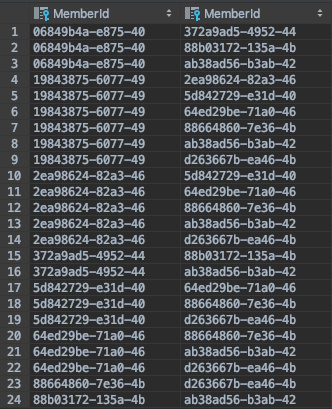
\includegraphics[scale=0.5]{Images/UserPairs-Board}
\end{figure}
\begin{lstlisting}[language=SQL, caption=Find Users Who Share At Least One Board]
SELECT DISTINCT A.MemberId, B.MemberId FROM BoardMember AS A INNER JOIN BoardMember as B ON A.BoardId = B.BoardId AND B.MemberId > A.MemberId;
\end{lstlisting}
\hrule
\begin{figure}[H]
\centering
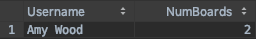
\includegraphics[scale=0.5]{Images/BoardsForUser}
\end{figure}
\begin{lstlisting}[language=SQL, caption=Select Board Membership for User "Amy Wood"]
SELECT Username, Count(*) as NumBoards FROM BoardMember INNER JOIN ApplicationUser on BoardMember.MemberId = ApplicationUser.Id WHERE Username = 'Amy Wood' GROUP BY Username;
\end{lstlisting}
\hrule
\begin{figure}[H]
\centering
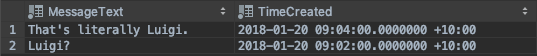
\includegraphics[scale=0.5]{Images/CommentsForUser}
\end{figure}
\begin{lstlisting}[language=SQL, caption=Select 10 Most Recent Comments for User "Phillip Ramirez"]
SELECT TOP 10 MessageText, TimeCreated FROM Comment INNER JOIN ApplicationUser on ApplicationUser.Id = Comment.OwnerId WHERE Username = 'Phillip Ramirez' ORDER BY TimeCreated DESC;
\end{lstlisting}
\hrule
\begin{figure}[H]
\centering
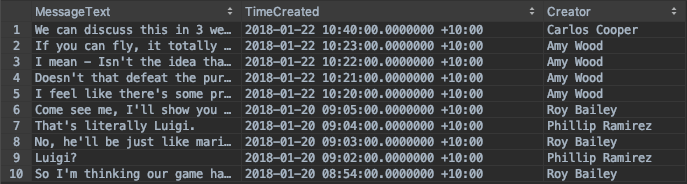
\includegraphics[scale=0.5]{Images/CommentsAllUsers}
\end{figure}
\begin{lstlisting}[language=SQL, caption=Select 10 Most Recent Comments]
SELECT TOP 10 MessageText, TimeCreated, Username as Creator FROM Comment, ApplicationUser WHERE ApplicationUser.Id = Comment.OwnerId ORDER BY TimeCreated DESC;
\end{lstlisting}
\hrule
\begin{figure}[H]
\centering
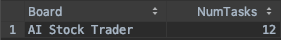
\includegraphics[scale=0.5]{Images/MostActiveBoard-Tasks}
\end{figure}
\begin{lstlisting}[language=SQL, caption=Select Most Active Board (Tasks)]
SELECT TOP 1 Board.Title as Board, COUNT(*) as NumTasks FROM Task INNER JOIN List ON Task.ListId = List.Id INNER JOIN Board on List.BoardId = Board.Id GROUP BY Board.Title ORDER BY NumTasks DESC;
\end{lstlisting}
\hrule
\begin{figure}[H]
\centering
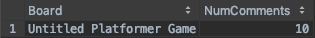
\includegraphics[scale=0.5]{Images/MostActiveBoard-Comments}
\end{figure}
\begin{lstlisting}[language=SQL, caption=Select Most Active Board (Comments)]
SELECT TOP 1 Board.Title as Board, COUNT(*) as NumComments FROM Comment INNER JOIN Task on Comment.TaskId = Task.Id INNER JOIN List ON Task.ListId = List.Id INNER JOIN Board on List.BoardId = Board.Id GROUP BY Board.Title ORDER BY NumComments DESC;
\end{lstlisting}
\hrule
\begin{figure}[H]
\centering
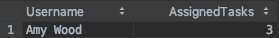
\includegraphics[scale=0.5]{Images/MostActiveUser-Tasks}
\end{figure}
\begin{lstlisting}[language=SQL, caption=Select Most Active User (Tasks)]
SELECT TOP 1 Username, COUNT(*) AS AssignedTasks FROM ApplicationUser INNER JOIN TaskAssignee on ApplicationUser.Id = TaskAssignee.AssigneeId GROUP BY Username ORDER BY AssignedTasks DESC;
\end{lstlisting}
\hrule
\begin{figure}[H]
\centering
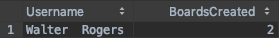
\includegraphics[scale=0.5]{Images/MostActiveUser-Boards}
\end{figure}
\begin{lstlisting}[language=SQL, caption=Select Most Active User (Boards)]
SELECT TOP 1 Username, COUNT(*) AS BoardsCreated FROM ApplicationUser INNER JOIN Board on ApplicationUser.Id = Board.OwnerId GROUP BY Username ORDER BY BoardsCreated DESC;
\end{lstlisting}
\hrule
\begin{figure}[H]
\centering
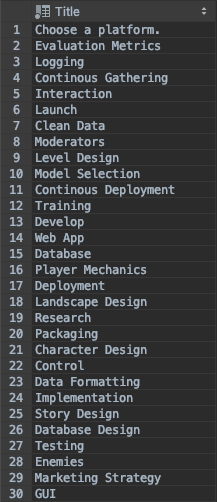
\includegraphics[scale=0.5]{Images/OverdueTasks}
\end{figure}
\begin{lstlisting}[language=SQL, caption=Select All Overdue Tasks]
SELECT Id FROM Task WHERE DueDate < SYSDATETIMEOFFSET();
\end{lstlisting}


\subsubsection{Other Statements}

\subsubsection{Update statements}

\section{Index}
\lstlistoflistings

\end{document}
